\section{Risultati dell'algoritmo \texttt{Karger}}
Questa sezione risponderà alle varie domande poste per l'assignement.

\subsection{Domanda 1}
Misurate i tempi di calcolo della procedura \texttt{full\_contraction} sui grafi del dataset. Mostrate i risultati con un grafico che mostri la variazione dei tempi di calcolo al variare del numero di vertici nel grafo. Confrontate i tempi misurati con la complessità asintotica di \texttt{full\_contraction}.

\subsubsection{Svolgimento}

\begin{center}
	\begin{longtable}{|c|c|c|}	
		\hline
		\textbf{N.} & \textbf{Size} & \textbf{Full Contraction Time (s)} \\ \hline
		\endfirsthead
		\multicolumn{3}{|c|}{\tablename\ \thetable\ \ --\  \textit{continuazione dalla pagina precedente}} \\
		\hline
		\textbf{N.} & \textbf{Size} & \textbf{Full Contraction Time (s)} \\ \hline
		\endhead
		\hline \multicolumn{3}{|c|}{\textit{Continua nella pagina seguente}} \\
		\endfoot  
		\endlastfoot
		\hline
		1 &	6 & 1.0E-6\\
		2 &	6 & 1.2E-6\\
		3 &	6 & 1.7E-6\\
		4 &	6 & 1.5E-6\\
		5 &	10 & 3.9E-6\\
		6 &	10 & 3.6E-6\\
		7 &	10 & 3.7E-6\\
		8 &	10 & 3.9E-6\\
		9 &	25 & 2.72E-5\\
		10 & 25	& 5.16E-5\\
		11 & 25	& 2.3E-5\\
		12 & 25	& 2.3E-5\\
		13 & 50	& 1.269E-4\\
		14 & 50	& 1.207E-4\\
		15 & 50	& 1.136E-4\\
		16 & 50	& 1.178E-4\\
		17 & 75	& 3.101E-4\\
		18 & 75	& 3.266E-4\\
		19 & 75	& 3.47E-4\\
		20 & 75	& 3.348E-4\\
		21 & 100 & 6.926E-4\\
		22 & 100 & 7.199E-4\\
		23 & 100 & 7.257E-4\\
		24 & 100 & 7.237E-4\\
		25 & 125 & 0.0014224\\
		26 & 125 & 0.0014538\\
		27 & 125 & 0.0015773\\
		28 & 125 & 0.0014295\\
		29 & 150 & 0.0030876\\
		30 & 150 & 0.0028798\\
		31 & 150 & 0.0029867\\
		32 & 150 & 0.0030172\\
		33 & 175 & 0.0046466\\
		34 & 175 & 0.0044992\\
		35 & 175 & 0.0052528\\
		36 & 175 & 0.0046107\\
		37 & 200 & 0.0072138\\
		38 & 200 & 0.0066759\\
		39 & 200 & 0.0072141\\
		40 & 200 & 0.0075121\\
		\hline
		\caption{Risultati della procedura \textit{Full Contraction} rispetto alla domanda 1}
		\label{fc-results}
	\end{longtable}
\end{center}\vspace{-40pt}

\begin{figure}[H]
	\centering
	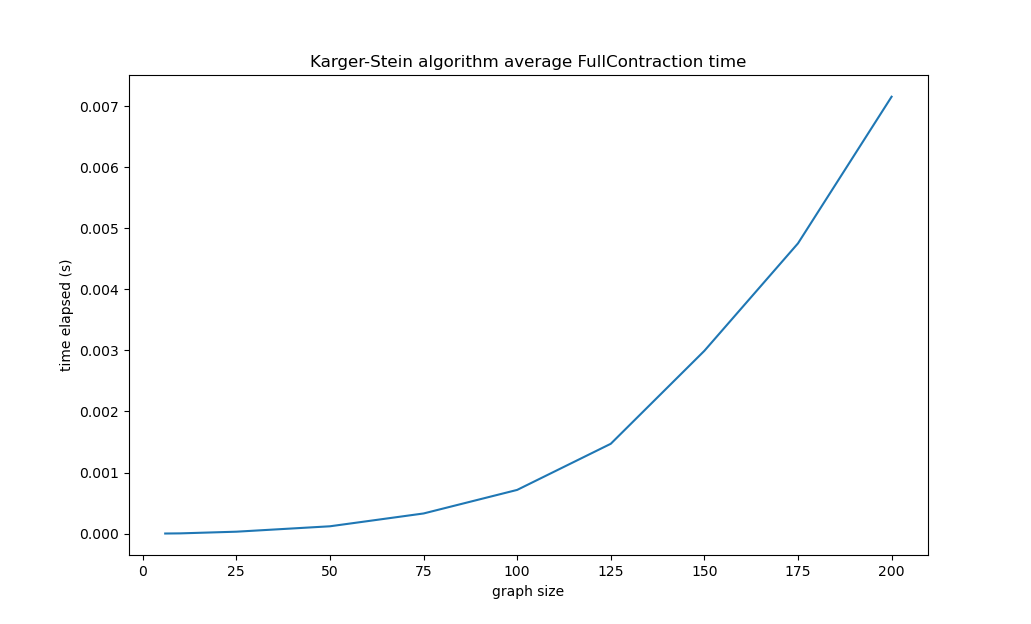
\includegraphics[width=\textwidth]{avg_fc_time}
	\caption{Analisi asintotica di \texttt{full\_contraction}}
	\label{fc-confronto}
\end{figure}

\texttt{full\_contraction} ha una complessità di \comp{n^2}, che è ben visibile dal grafico in Figura 3.

\subsection{Domanda 2}
Misurate i tempi di calcolo dell'algoritmo di Karger sui grafi del dataset, usando un numero di ripetizioni che garantisca una probabilità minore o uguale a $\frac{1}{n}$ di sbagliare. Mostrate i risultati con un grafico che mostri la variazione dei tempi di calcolo al variare del numero di vertici nel grafo. Confrontate i tempi misurati con la complessità asintotica dell'algoritmo.

\subsubsection{Svolgimento}
\subsubsection*{Calcolo del numero di iterazioni necessarie}
\begin{itemize}
	\item Analisi di una singola iterazione di FC.\vspace{-5pt}
	\begin{itemize}
		\item Sia $t = |$ min-cut $| = C$
		\item $E_i = $ al passo $i-$esimo di FC;
		\item $Pr($successo di FC\footnote{cioè non becco nessun arco di taglio minimo $C$})$\,\geq Pr\left(\mathlarger{\bigcap}_{i=1}^{n-2} E_1\right)$.\\
		\begin{itemize}
		\item $Pr(E_1) \geq 1- \frac{t}{t\frac{n}{2}} = 1 - \dfrac{2}{n}$. Quindi la probabilità di non beccare un arco del min-cut alla prima iterazione di FC è buona. Successo con alta probabilità.
		\item $Pr(E_2|E_1) \geq 1 - \dfrac{t}{t \frac{n-1}{2}}$
		\item $\quad\vdots$
		\item $Pr(E_i|E_1\cap E_2\cap ...\cap E_{i-1}) \geq 1 - \dfrac{t}{t \frac{(n-i+1)}{2}} = 1 - \dfrac{2}{n-i+1}$
		\end{itemize}
		$\Rightarrow Pr($successo di FC$) \geq Pr\left(\mathlarger{\bigcap}_{i=1}^{n-2} E_1\right) \geq \mathlarger{\prod}_{i=1}^{n-2}\left(1 - \dfrac{2}{n-i+1}\right) = Pr\left(\mathlarger{\bigcap}_{i=1}^{n-2} E_1\right) \dfrac{n-i-1}{n-i+1} =$\eqcapo 
		$ = \dfrac{(n-2)}{n}\cdot\dfrac{(n-3)}{n-1}\cdot\dfrac{(n-4)}{n-2}\cdot\,\cdots\,\cdot\dfrac{3}{5}\cdot\dfrac{2}{4}\cdot\dfrac{1}{3} = \dfrac{2}{n(n-1)} \geq \dfrac{2}{n^2}$\eqcapo
		Quindi, eseguendo FC una sola volta, la probabilità di non beccare un arco appartenente al min-cut è almeno di $\dfrac{2}{n^2}$. 
		\end{itemize}
		\item Dobbiamo calcolare la probabilità che le $k$ iterazioni di FC non accumulino la taglia del min-cut.
	\begin{itemize}
		\item $Pr($le $k$ FC non accumulano la taglia del min-cut$) \leq \left(1 - \dfrac{2}{n^2}\right)^k$ (evento insuccesso)\\
		Vogliamo che questa probabilità sia $\leq \dfrac{1}{n}$. Quindi scelgo $k =\dfrac{n^2}{2}\log n$. Dimostriamo che è sufficiente.
		\begin{itemize}
			\item Infatti 
			$\left(\left( 1- \dfrac{2}{n^2}\right)^{\frac{n^2}{2}}\right)^{\log n} \leq e^{-\log n} = \dfrac{1}{n}$.
		\end{itemize}
	\end{itemize}
	\item Quindi con probabilità almeno $\dfrac{1}{n}$ l'algoritmo di Karger accumula la taglia del min-cut.
\end{itemize}
\begin{center}
	\begin{longtable}{|c|c|c|c|}	
		\hline
		\textbf{N.} & \textbf{Size} & \textbf{Karger solution} & \textbf{Karger Time (s)}
		\endfirsthead
		\multicolumn{4}{|c|}{\tablename\ \thetable\ \ --\  \textit{continuazione dalla pagina precedente}} \\ \hline
		\textbf{N.} & \textbf{Size} & \textbf{Karger solution} & \textbf{Karger Time (s)} \\ \hline
		\endhead \hline 
		\multicolumn{4}{|c|}{\textit{Continua nella pagina seguente}} \\
		\endfoot  
		\endlastfoot
		\hline
		1 & 6 & 2 & 4.59E-5 \\
		2 & 6 & 1 & 4.97E-5 \\
		3 & 6 & 3 & 5.39E-5 \\
		4 & 6 & 4 & 5.37E-5 \\
		5 & 10 & 4 & 5.103E-4 \\
		6 & 10 & 3 & 4.918E-4 \\
		7 & 10 & 2 & 4.965E-4 \\
		8 & 10 & 1 & 4.971E-4 \\
		9 & 25 & 7 & 0.0306304 \\
		10 & 25 & 6 & 0.0957754 \\		
		11 & 25 & 8 & 0.0318386 \\		
		12 & 25 & 9 & 0.0320083 \\		
		13 & 50 & 15 & 0.7410805 \\		
		14 & 50 & 16 & 0.7322812 \\		
		15 & 50 & 14 & 0.6886227 \\		
		16 & 50 & 10 & 0.7194658 \\		 
		17 & 75 & 19 & 4.5581846 \\		
		18 & 75 & 15 & 4.7667614 \\		
		19 & 75 & 18 & 4.7321971 \\		
		20 & 75 & 16 & 4.6194424 \\		
		21 & 100 & 22 & 18.4590746 \\		
		22 & 100 & 23 & 18.3235051 \\		
		23 & 100 & 19 & 19.2442024 \\		
		24 & 100 & 24 & 19.2161447 \\		
		25 & 125 & 34 & 58.8190144 \\		
		26 & 125 & 29 & 57.457255 \\		
		27 & 125 & 36 & 70.1068629 \\		
		28 & 125 & 31 & 58.5128556 \\		
		29 & 150 & 37 & 164.4596518 \\		
		30 & 150 & 35 & 159.8519787 \\		 	
		31 & 150 & 41 & 164.7340277 \\		
		32 & 150 & 39 & 162.4446075 \\		
		33 & 175 & 42 & 354.6868445 \\		
		34 & 175 & 45 & 355.8195941 \\		 
		35 & 175 & 53 & 376.6771329 \\		   
		36 & 175 & 43 & 339.6508817 \\		
		37 & 200 & 54 & 730.3265273 \\		
		38 & 200 & 52 & 685.7037242 \\		
		39 & 200 & 51 & 708.7966211 \\		
		40 & 200 & 61 & 730.9270492 \\			
		\hline
		\caption{Risultati della procedura \textit{Karger} rispetto alla domanda 2}
		\label{k-results}
	\end{longtable}
\end{center}\vspace{-40pt}

\begin{figure}[H]
	\centering
	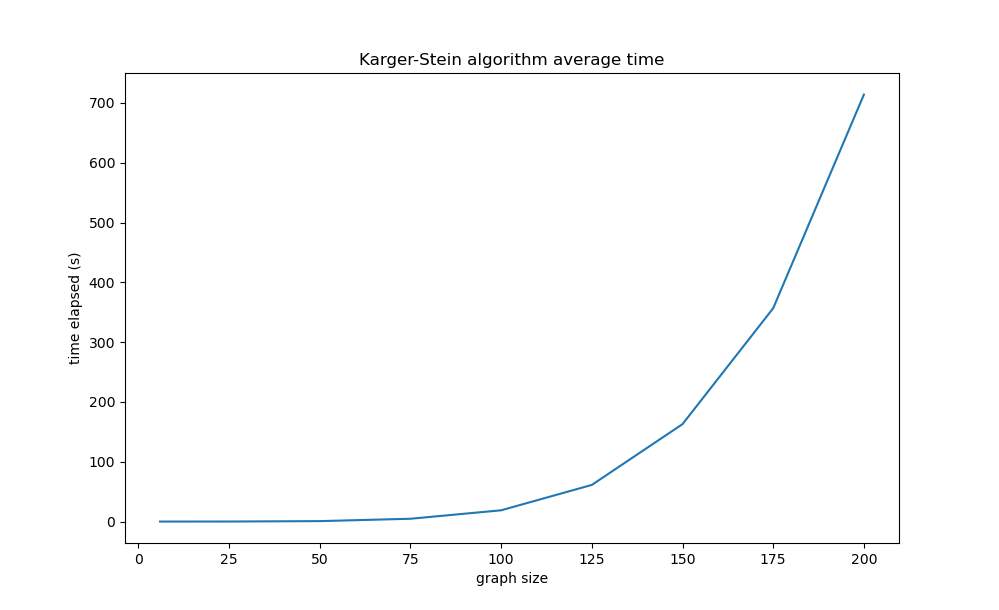
\includegraphics[width=\textwidth]{avg_time}
	\caption{Analisi asintotica di \texttt{Karger}}
	\label{k-confronto}
\end{figure}

La procedura \texttt{Karger} ha una complessità di\comp{n^4 \log n}, infatti è possibile vedere in Figura 4 come rispetto a Figura 3\footnote{che si riferisce ad una curva asintotica di \comp{n^2}} la curva inizia ad impennarsi fin da subito ma in modo più ripido.

\begin{figure}[H]
	\centering
	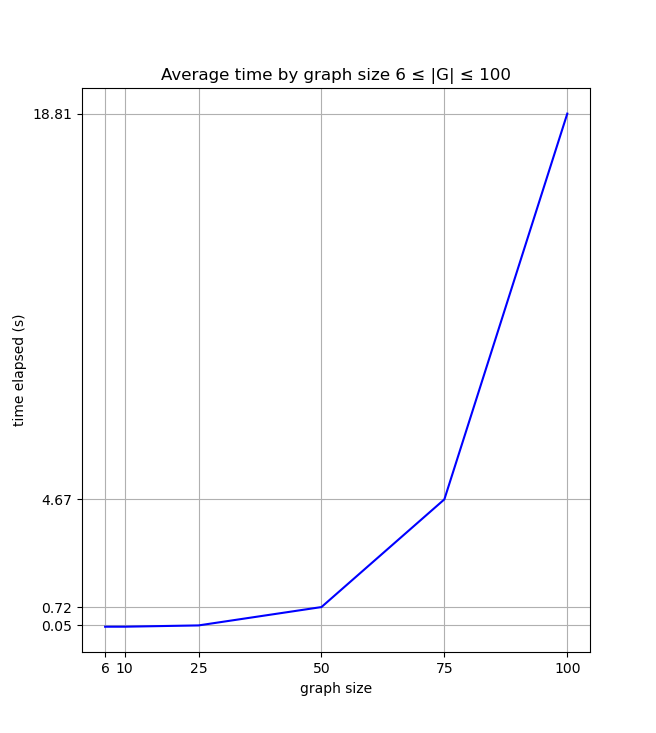
\includegraphics[width=0.8\textwidth]{avg_time_6-100}
	\caption{Analisi asintotica di \texttt{Karger} per i grafi da 6 a 100 nodi}
	\label{k-confronto1}
\end{figure}

\begin{figure}[H]
	\centering
	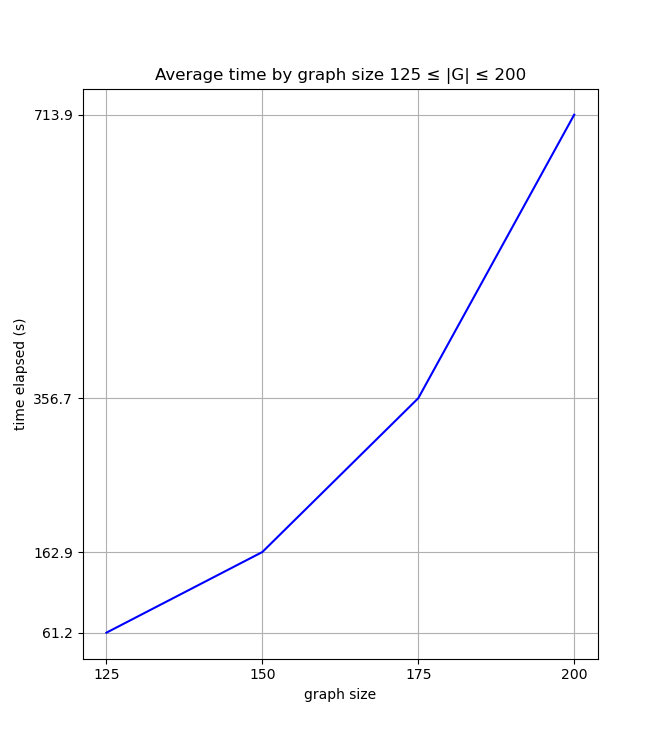
\includegraphics[width=0.8\textwidth]{avg_time_125-200}
	\caption{Analisi asintotica di \texttt{Karger} per i grafi da 125 a 200 nodi}
	\label{k-confronto2}
\end{figure}

La procedura \texttt{Karger} ha una complessità di\comp{n^4 \log n}, che è possibile analizzare molto bene attraverso Figura~\ref{k-confronto1} e Figura~\ref{k-confronto2}. Infatti è molto evidente come la curva dei grafici si impenni molto più velocemente rispetto \texttt{full\_contraction} in Figura~\ref{fc-confronto}.

\subsection{Domanda 3}
Misurate il \textit{discovery time} dell'algoritmo di Karger sui grafi del dataset. Il discovery time è il momento (in secondi) in cui l'algoritmo trova per la prima volta il taglio di costo mimimo.  Confrontate il discovery time con il tempo di esecuzione complessivo per ognuno dei grafi nel dataset.

\subsubsection{Svolgimento}

\begin{center}
	\begin{longtable}{|c|c|c|c|}	
		\hline
		\textbf{N.} & \textbf{Size} & \textbf{Karger Tme (s)} & \textbf{Discovery Time (s)} \\ \hline
		\endfirsthead
		\multicolumn{4}{|c|}{\tablename\ \thetable\ \ --\  \textit{continuazione dalla pagina precedente}} \\ \hline
		\textbf{N.} & \textbf{Size} & \textbf{Karger Time (s)} & \textbf{Discovery Time (s)}
		\endhead
		\hline \multicolumn{4}{|c|}{\textit{Continua nella pagina seguente}} \\ 
		\endfoot  
		\endlastfoot
		\hline
		1 & 6 & 4.59E-5	 & 1.26E-5 \\			    
		2 & 6 & 4.97E-5	 & 3.7E-6 \\			   	
		3 & 6 & 5.39E-5	 & 9.7E-6 \\		   		
		4 & 6 & 5.37E-5	 & 3.2E-6 \\			    
		5 & 10 & 5.103E-4 & 1.284E-4 \\	   		
		6 & 10 & 4.918E-4 & 5.8E-6 \\			  	
		7 & 10 & 4.965E-4 & 2.75E-5 \\			    
		8 & 10 & 4.971E-4 & 5.9E-6 \\			   	
		9 & 25 & 0.0306304 & 7.73E-4 \\
		10 & 25 & 0.0957754 & 0.0115143 \\		   	
		11 & 25 & 0.0318386 & 0.0077459 \\			
		12 & 25 & 0.0320083 & 0.0040907 \\	  		
		13 & 50 & 0.7410805 & 0.0138128 \\		    
		14 & 50 & 0.7322812 & 0.0478224 \\	    	
		15 & 50 & 0.6886227 & 0.003738 \\	  		
		16 & 50 & 0.7194658 & 0.0149178 \\	        
		17 & 75 & 4.5581846 & 0.0762589 \\	   		
		18 & 75 & 4.7667614 & 0.0404856 \\	  		
		19 & 75 & 4.7321971 & 0.0265994 \\	   		
		20 & 75 & 4.6194424 & 0.1123946 \\		  	
		21 & 100 & 18.4590746 & 0.1588621 \\	 
		22 & 100 & 18.3235051 & 0.0822596 \\	 
		23 & 100 & 19.2442024 & 0.0168746 \\		 
		24 & 100 & 19.2161447 & 0.0251183 \\		 
		25 & 125 & 58.8190144 & 0.4463958 \\	  
		26 & 125 & 57.457255 & 0.1294754 \\		
		27 & 125 & 70.1068629 & 1.0395953 \\		 
		28 & 125 & 58.5128556 & 0.8252303 \\		 
		29 & 150 & 164.4596518 & 6.6862347 \\	  
		30 & 150 & 159.8519787 & 0.9646022 \\	    
		31 & 150 & 164.7340277 & 0.5240023 \\		 
		32 & 150 & 162.4446075 & 6.4803055 \\		 
		33 & 175 & 354.6868445 & 3.0379762 \\		 
		34 & 175 & 355.8195941 & 1.7371626 \\	   	
		35 & 175 & 376.6771329 & 22.2364104 \\	  	 
		36 & 175 & 339.6508817 & 2.4007981 \\	 
		37 & 200 & 730.3265273 & 7.7587212 \\		 
		38 & 200 & 685.7037242 & 0.6157363 \\	  
		39 & 200 & 708.7966211 & 3.3346295 \\	  
		40 & 200 & 730.9270492 & 12.4704872 \\	
		\hline
		\caption{Risultati della procedura \textit{Karger} rispetto alla domanda 3}
		\label{dt-results}
	\end{longtable}
\end{center}\vspace{-40pt}

\begin{figure}[H]
	\centering
	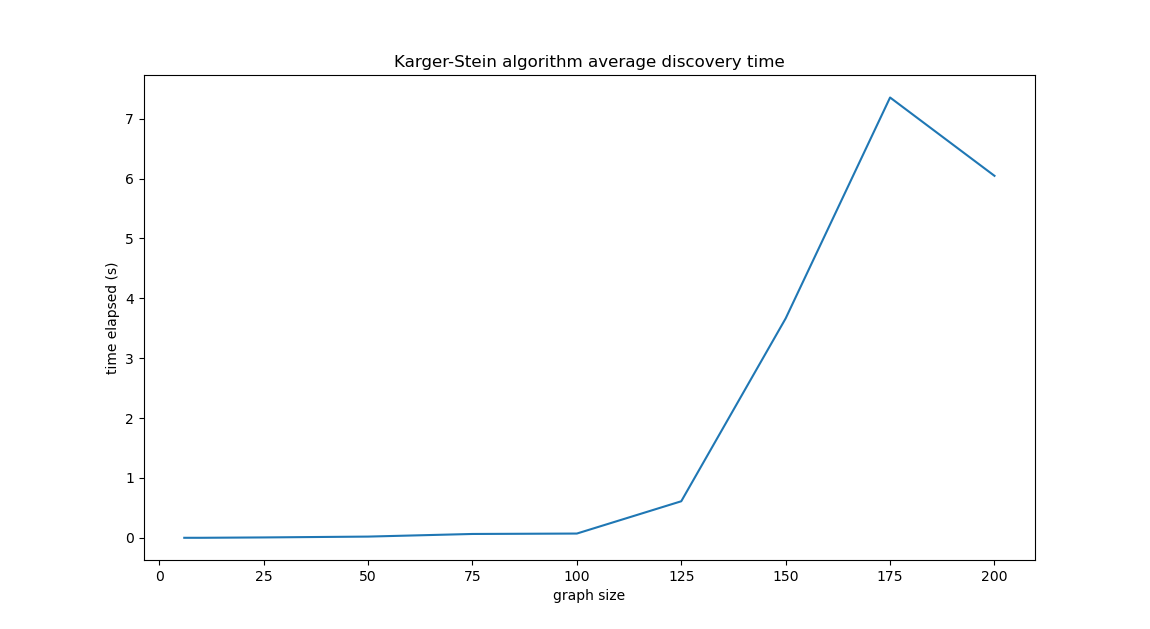
\includegraphics[width=\textwidth]{avg_disc_time}
	\caption{Analisi del \texttt{discovery\_time}}
	\label{dt-confronto}
\end{figure}

Dato che l'algoritmo di Karger è un algoritmo randomizzato, non è possibile determinare quando e se otterrà la soluzione corretta, dunque è normale che in Figura~\ref{dt-confronto} l'andamento non sia regolare.\\
\'E importante invece notare come il \textit{discovery\_time} sia in generale almeno 10 volte minore del tempo di esecuzione di \texttt{Kager}, questo vuol dire che la soluzione corretta viene trovata già prima delle $\frac{k}{10}$ iterazioni, con $k = n^2 \log n$. Da ciò si può dedurre che già dopo $\frac{k}{10}$ iterazioni la probabilità di trovare la soluzione corretta è già molto alta.\\
In particolare è interessante vedere in Figura~\ref{dt-confronto1}, Figura~\ref{dt-confronto2}, Figura~\ref{dt-confronto3} e Figura~\ref{dt-confronto4} la differenza tra \textit{discovery\_time} ed il tempo di esecuzione di \texttt{Karger} e di come il \textit{discovery\_time} sembri quasi lineare, rispetto a \texttt{Karger} che invece è esponenziale.

\begin{figure}[H]
	\centering
	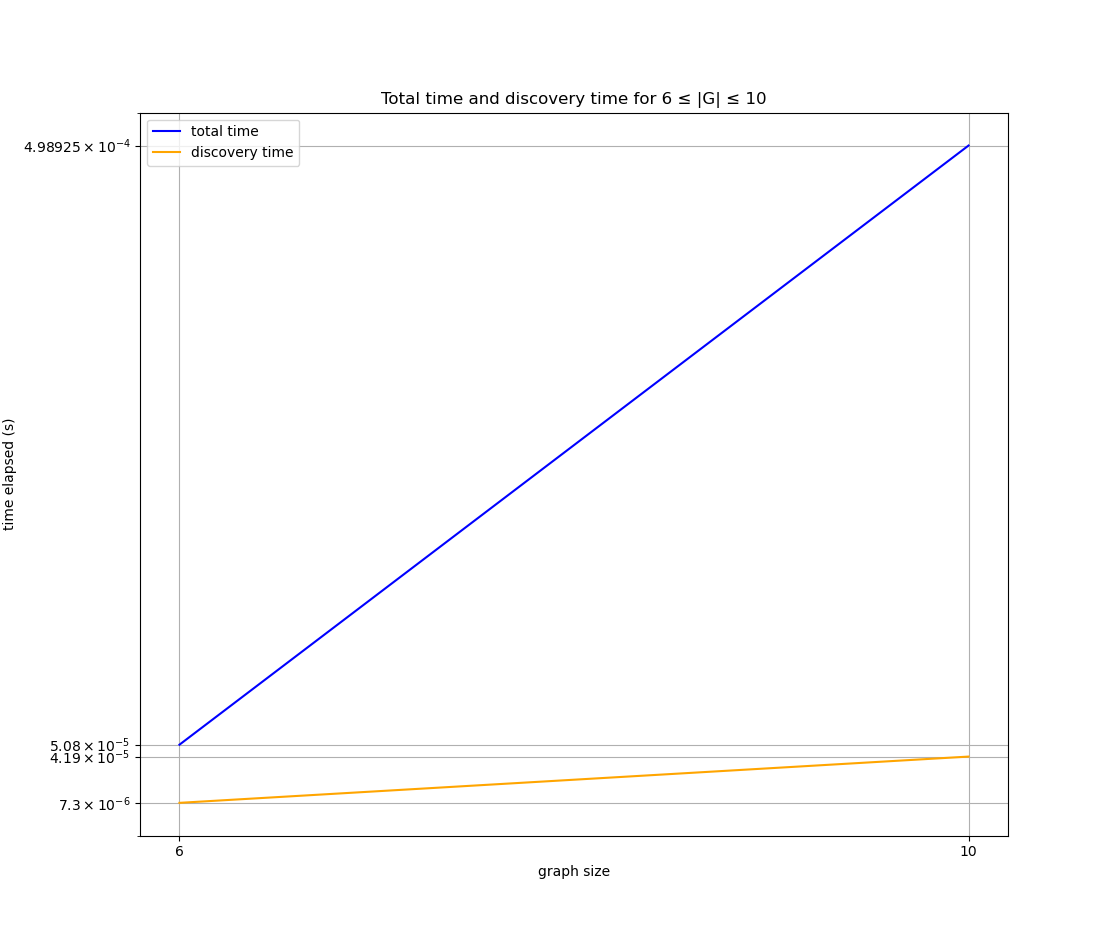
\includegraphics[width=\textwidth]{tot_disc_6-10}
	\caption{Analisi del \texttt{discovery\_time}}
	\label{dt-confronto1}
\end{figure}

\begin{figure}[H]
	\centering
	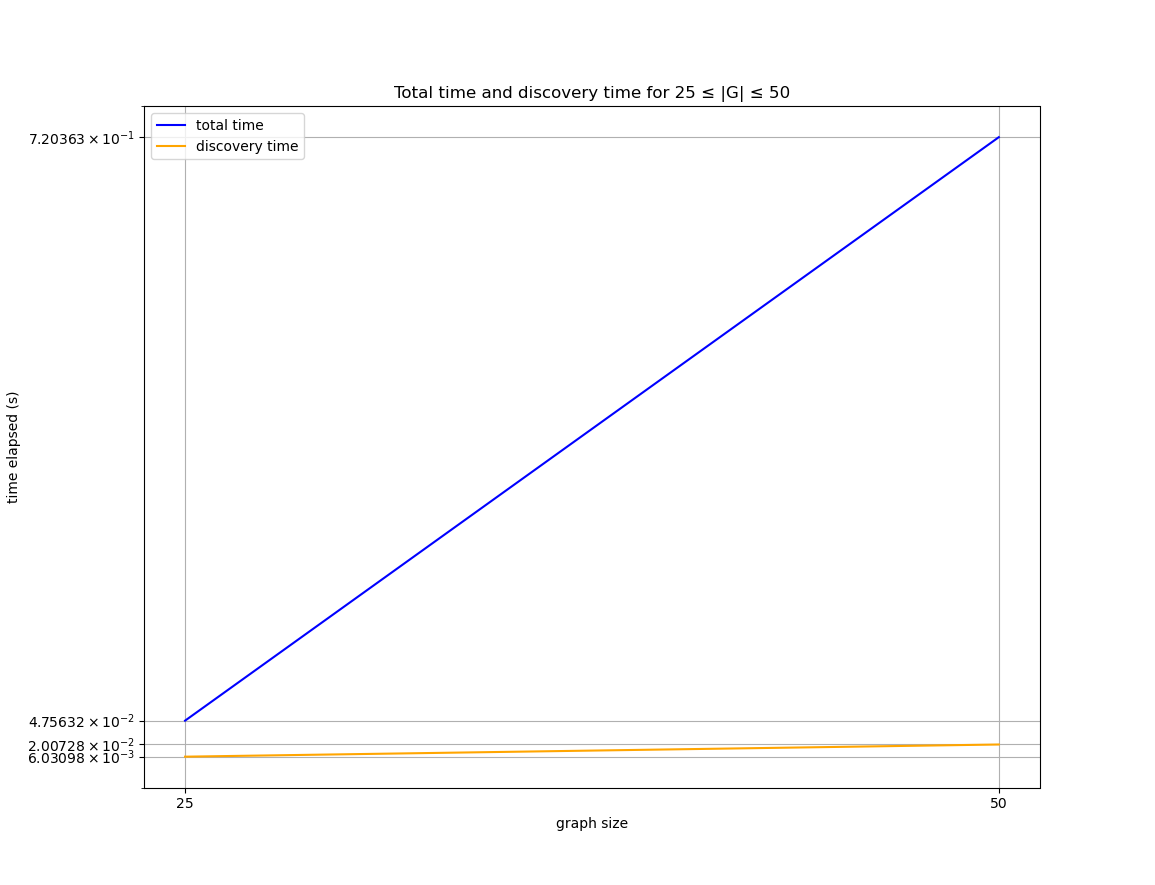
\includegraphics[width=\textwidth]{tot_disc_25-50}
	\caption{Analisi del \texttt{discovery\_time}}
	\label{dt-confronto2}
\end{figure}

\begin{figure}[H]
	\centering
	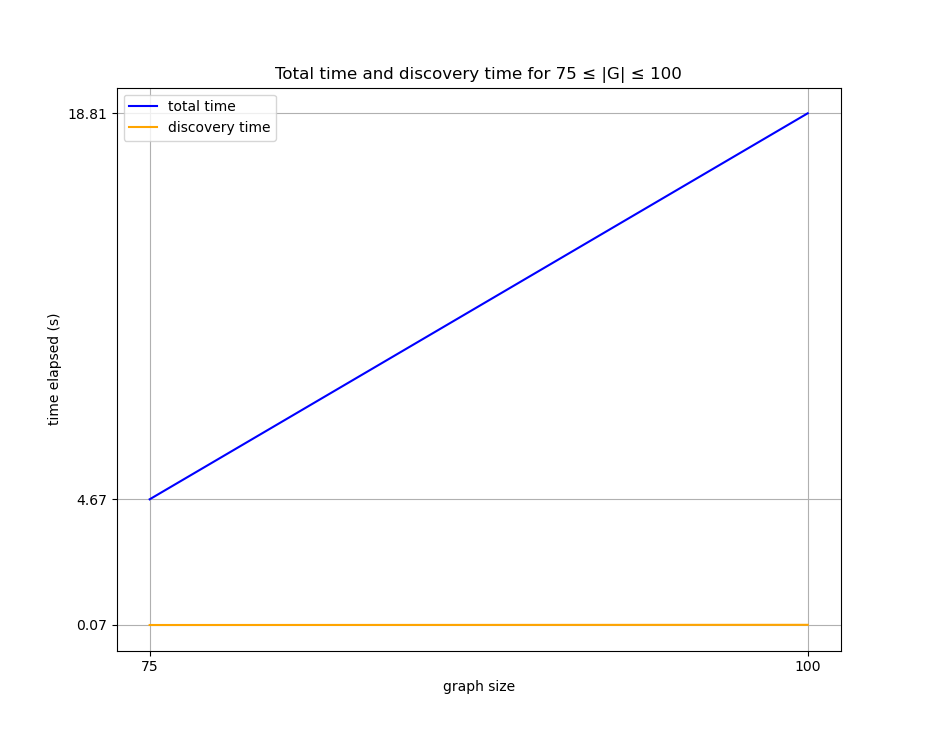
\includegraphics[width=\textwidth]{tot_disc_75-100}
	\caption{Analisi del \texttt{discovery\_time}}
	\label{dt-confronto3}
\end{figure}

\begin{figure}[H]
	\centering
	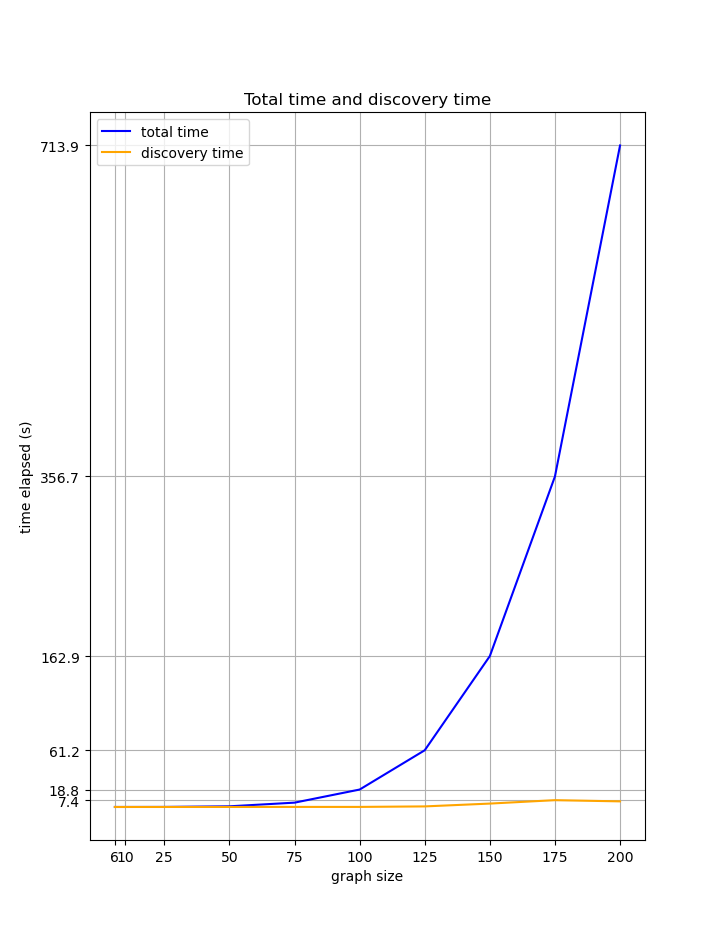
\includegraphics[width=\textwidth]{tot_disc_all}
	\caption{Analisi del \texttt{discovery\_time}}
	\label{dt-confronto4}
\end{figure}

\subsection{Domanda 4}
Per ognuno dei grafi del dataset, riportate il risultato risultato ottenuto dalla vostra implementazione, la soluzione attesa e l'errore relativo calcolato come $ \frac{\textrm{SoluzioneTrovata}-\textrm{SoluzioneAttesa}}{\textrm{SoluzioneAttesa}}$.

\subsubsection{Svolgimento}

\begin{center}
	\begin{longtable}{|c|c|c|c|c|}	
		\hline
		\textbf{N.} & \textbf{Size} & \textbf{Karger Solution} & \textbf{Solution} & \textbf{Error (\%)}
		\endfirsthead
		\multicolumn{5}{|c|}{\tablename\ \thetable\ \ --\  \textit{continuazione dalla pagina precedente}} \\
		\hline
		\textbf{N.} & \textbf{Size} & \textbf{Karger Solution} & \textbf{Solution} & \textbf{Error (\%)} \\ \hline
		\endhead
		\hline \multicolumn{5}{|c|}{\textit{Continua nella pagina seguente}} \\
		\endfoot  
		\endlastfoot
		\hline
		1 & 6 & 2 & 2 & 0.0 \\
		2 & 6 & 1 & 1 & 0.0 \\
		3 & 6 & 3 & 3 & 0.0 \\
		4 & 6 & 4 & 4 & 0.0 \\
		5 & 10 & 4 & 4 & 0.0 \\
		6 & 10 & 3 & 3 & 0.0 \\
		7 & 10 & 2 & 2 & 0.0 \\
		8 & 10 & 1 & 1 & 0.0 \\
		9 & 25 & 7 & 7 & 0.0 \\
		10 & 25 & 6 & 6 & 0.0 \\
		11 & 25 & 8 & 8 & 0.0 \\
		12 & 25 & 9 & 9 & 0.0 \\
		13 & 50 & 15 & 15 & 0.0 \\
		14 & 50 & 16 & 16 & 0.0 \\
		15 & 50 & 14 & 14 & 0.0 \\
		16 & 50 & 10 & 10 & 0.0 \\
		17 & 75 & 19 & 19 & 0.0 \\
		18 & 75 & 15 & 15 & 0.0 \\
		19 & 75 & 18 & 18 & 0.0 \\
		20 & 75 & 16 & 16 & 0.0 \\
		21 & 100 & 22 & 22 & 0.0 \\
		22 & 100 & 23 & 23 & 0.0 \\
		23 & 100 & 19 & 19 & 0.0 \\
		24 & 100 & 24 & 24 & 0.0 \\
		25 & 125 & 34 & 34 & 0.0 \\
		26 & 125 & 29 & 29 & 0.0 \\
		27 & 125 & 36 & 36 & 0.0 \\
		28 & 125 & 31 & 31 & 0.0 \\
		29 & 150 & 37 & 37 & 0.0 \\
		30 & 150 & 35 & 35 & 0.0 \\
		31 & 150 & 41 & 41 & 0.0 \\
		32 & 150 & 39 & 39 & 0.0 \\
		33 & 175 & 42 & 42 & 0.0 \\
		34 & 175 & 45 & 45 & 0.0 \\
		35 & 175 & 53 & 53 & 0.0 \\
		36 & 175 & 43 & 43 & 0.0 \\
		37 & 200 & 54 & 54 & 0.0 \\
		38 & 200 & 52 & 52 & 0.0 \\
		39 & 200 & 51 & 51 & 0.0 \\
		40 & 200 & 61 & 61 & 0.0 \\
		\hline
		\caption{Risultati della procedura \textit{Karger} rispetto alla domanda 4}
		\label{error-results}
	\end{longtable}
\end{center}\vspace{-40pt}

Abbiamo deciso di eseguire l'algoritmo di Karger senza alcun tipo di timeout, dato che coi grafi più grandi richiedeva neanche 15 minuti di tempo, e per tutti i grafi la soluzione corretta è stata trovata, avendo dunque un errore relativo sempre dello 0\%.

\section{Conclusioni}
Nella realizzazione dell'elaborato abbiamo riscontrato qualche difficoltà nel cercare di capire quale fosse il modello per rappresentare i grafi più efficiente per eseguire l'algoritmo di Karger, in particolar modo per quanto riguardava la fase di contrazione dei lati, dato che quest'ultima doveva essere \comp{n}. Abbiamo dunque deciso di creare un modello che occupasse più memoria, attraverso le matrici di adiacenza, in favore di una complessità migliore.\\
\'E stato inoltre interessante vedere come la soluzione ottima venisse trovata quasi sempre tra le prime $\frac{k}{10}$ iterazioni circa.\\
Ci riteniamo soddisfatti del lavoro svolto, poiché siamo riusciti ad evitare l'uso di un \textit{timeout}: questo ci fa capire che siamo riusciti a rispettare la complessità, trovando nel 100\% dei dataset forniti la soluzione aspettata in tempi relativamente brevi, all'incirca 12 minuti per i grafi più grandi da 200 nodi.